\chapter{Electromagnetic simulations on analytic geometries}

\section{Slab configurations}
\subsection{Analysis of a plasma blob}
\label{ssec:plasmablob}

The linear analysis from the previous section has only , as characteristic shear Alfvén and thermal electron times are much shorter than the ion cyclotronic time, which underlies the resolution of typical turbulent SOLEDGE3X simulations. Drift Alfvén waves in turn correspond to the impact of inductive electromagnetic effect on the formation of drift waves, where the term $\partial_t A_\parallel$ in Ohm's law (Eq. \ref{eq:ParallelCurrent}) modifies the non-adiabatic response of the potential $\Phi$ to parallel fluctuations of the electron pressure $p_e$. To study the these effects on a plasma blob in a slab domain. \newline

We place ourselves in a plasma environment similar to the separatrix region in the diverted TCV simulations from the next Sec. \ref{sec:TCVsimulations}. The magnetic field is aligned to the toroidal coordinate with $B_{eq,t} = 1.3$T with a curvature of $1.1$m from the tokamak center, similar to the position of the separatrix at the outer mid-plane in TCV. Limiters are placed at both toroidal ends such that that connection length $L_\varphi = 65$m. A cartesian grid with coordinates $r$ and $z$ discretizes each poloidal plane, allowing radial fluxes out and with periodic boundary conditions in the vertical $z$-direction. The electron temperature is kept constant at $T_e=60$eV, ions are cold and the background density is set to $n_0 = 10^{19}$part/m$^3$. To simplify the study and prevent numerical difficulties at the sheath, we apply Neumann-0 boundary $\partial_\parallel n^{BC} = 0$ on the density and the potential $\Phi$ is fixed to $\Phi^{BC} = \Lambda T_e^{BC}$. This is a major simplification to the typical SOLEDGE3X sheath conditions described in Sec. \ref{sec:boundaryConditions}. The axisymmetric blob initially takes a Gaussian profile 
\begin{equation}
	n = n_0 \left(1 + \alpha e^{-\left[(r-r_b)^2+(z-z_b)^2\right]/\delta_b}\right)
	\label{eq:blobInitProfile}
\end{equation}
with a blob overdensity $\alpha = 2$ and radius $\delta_b = 1$cm. The blob evolves with curvature and electric drifts, neglecting anomalous perpendicular diffusion and viscous effects. Further, electron inertia effect are neglected with $m_e = 0$. We compare the reference electrostatic case with magnetic induction in the parallel electric field and the full electromagnetic setting including flutter. The simulation results are collected in Fig. \ref{fig:BLOB}. \newline

\begin{figure}[H]\centering
	\centering
	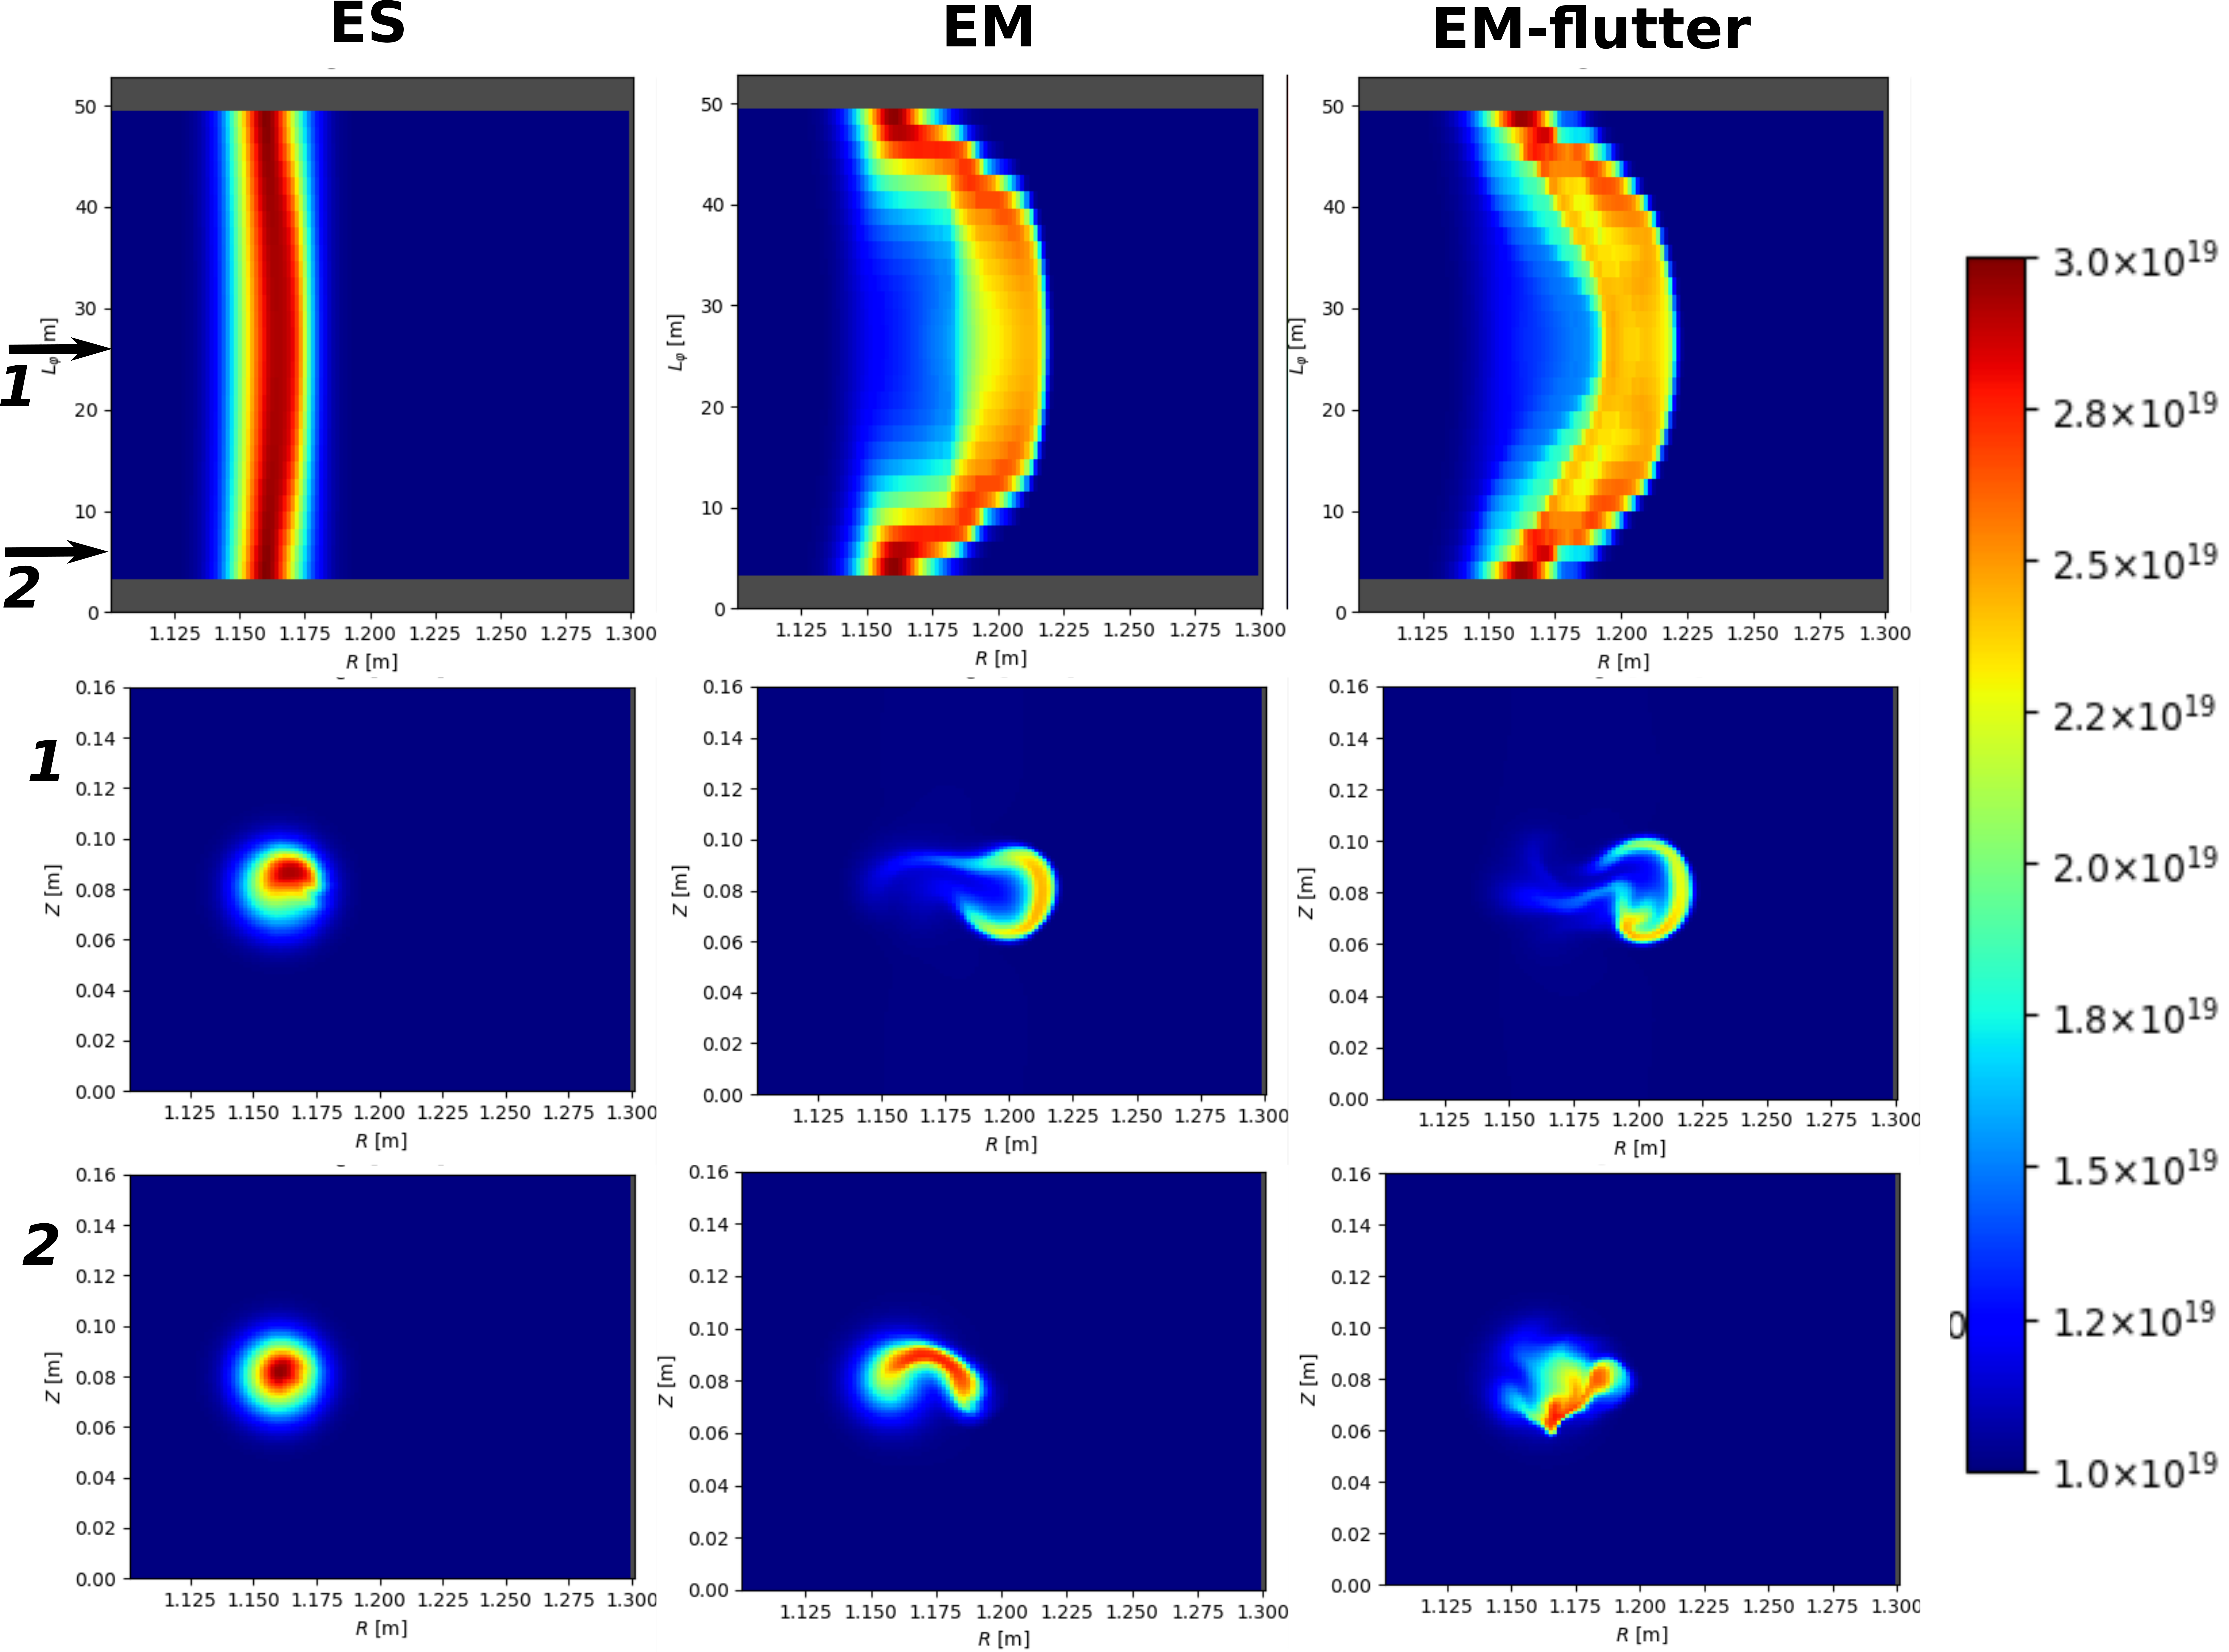
\includegraphics[width=1.\textwidth]{schemes/blob_compare_9_6_microsec.png}
	\caption{Density profiles [part/m³] after 9.6$\mu$s simulated plasma time for the electrostatic (ES), magnetic inductive (EM) and full electromagnetic scenarios (EM-flutter). The first row shows a view of the $R-\varphi$ plane with the maximum density taken along the $Z$ coordinate. The second and third rows show the density on poloidal planes ($R-Z$) at the center of the field lines (1) and in proximity to the sheath (2).}
	\label{fig:BLOB}
\end{figure}

In the center of the domain, drift waves determine the potential $\Phi$ but it is dominated by the sheath in proximity to the limiters. Hence a parallel gradient appears on $\Phi$, which in turn induces a parallel current responsive to inductive electromagnetic effects. As a result, the blob filaments bends along the toroidal direction, with higher advection velocities in the center of the domain than at the sheath. The bending is much more pronounced for the two electromagnetic scenarios, in line with the findings of previous blob studies\cite{lee2015,lee2015electromagnetic,Stepanenko_2020}. On closed field lines, the blob would conserve its axisymmetry and both $j_\parallel$ and $A_\parallel$ would remain 0 throughout the simulation. \newline




\subsection{Generation of drift waves}
\label{ssec:plasmaturbslab}

In the previous section, we examined how a single plasma blob propagates across open field lines. However, this does not account for how the blob appears in the first place. In this second part of the slab study, we investigate the onset of drift waves. We consider the same setting as before but with a background density of $n_0 = 2 \cdot 10^{19}$ part/m$^3$ and isothermal electrons and ions at $T_e = T_i = 50$ eV. Instead of an initial overdensity, we apply a constant particle source of $5 \cdot 10^{22}$ part/s on the core side, at all $R < 1.12$ m. The emergence of drift-wave instabilities for the three scenarios is shown in Fig. \ref{fig:SLABturb}. \newline

Initially, the particle source causes the density to build up on the core side of the slab. The radial gradient becomes stronger and soon collapses into drift waves. These waves are particularly pronounced in the electrostatic and electromagnetic inductive models. The term $\partial_t A_\parallel$ in Ohm's law intensifies the turbulent interchange, with plasma filaments reaching much further outward. On the other hand, the electromagnetic model with flutter has a stabilizing effect, producing only a thin turbulent layer at the exit of the source and maintaining a strong gradient at the transition from high- to low-density regions. As more particles are introduced at the source, the pressure differential causes this transition line to bend at scales of the simulation box, while the local gradient remains very steep. \newline

\begin{figure}[H]\centering
	\centering
	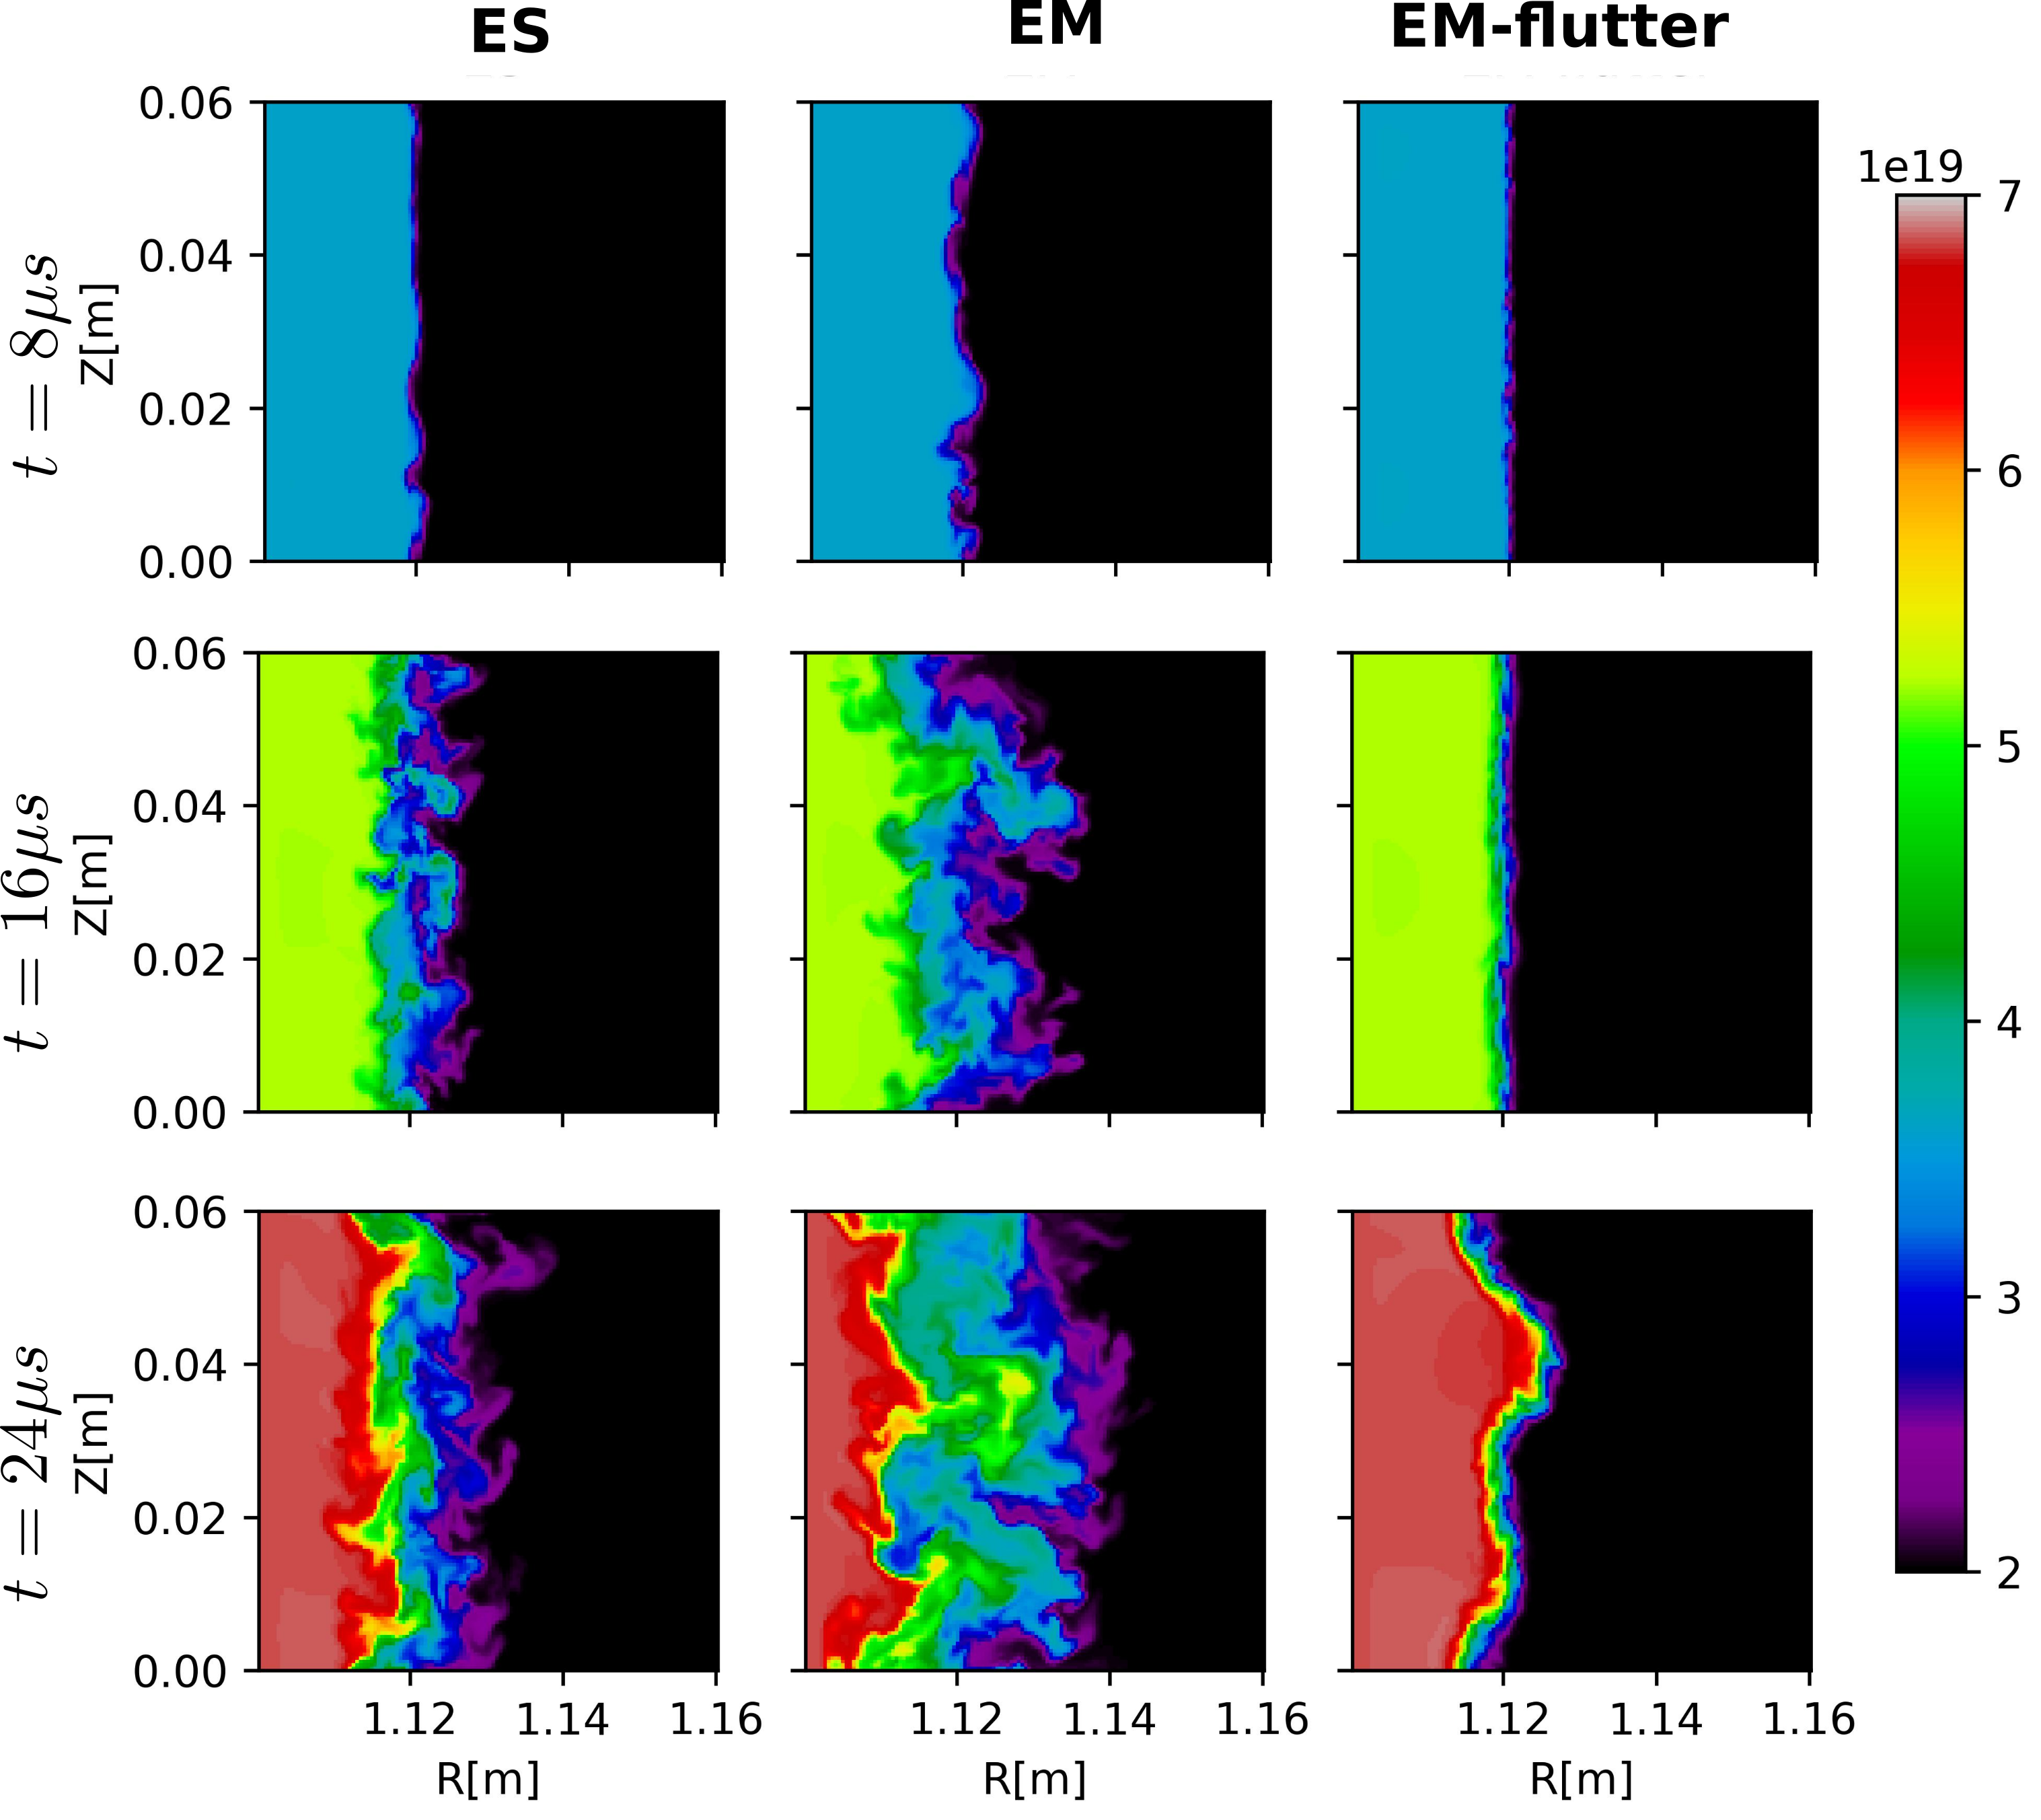
\includegraphics[width=.95\textwidth]{schemes/slab_source.png}
	\caption{Density profiles [part/m³] at the toroidal center of the slab, at about 32m from both limiters. The snapshots compare the electrostatic (ES), magnetic inductive (EM) and full electromagnetic scenarios (EM-flutter) scenarios after 8, 16 and 24$\mu$s simulated plasma time.}
	\label{fig:SLABturb}
\end{figure}


\section{Circular geometry}

\subsection{Simulation set-up}

Flat limiter on the low-field side


\begin{figure}[H]\centering
	\centering
	
\includegraphics[width=1\textwidth]{schemes/CIRC_fluctT.jpg}
	\caption{Snapshots of the electron temperature $T_e$ fluctuations}
	\label{fig:CIRC_fluctPHI}
\end{figure}


\subsection{Growth rates}


\subsubsection{Electron inertia}

\begin{figure}[H]\centering
	\begin{subfigure}[t]{0.45\textwidth}
		\centering
		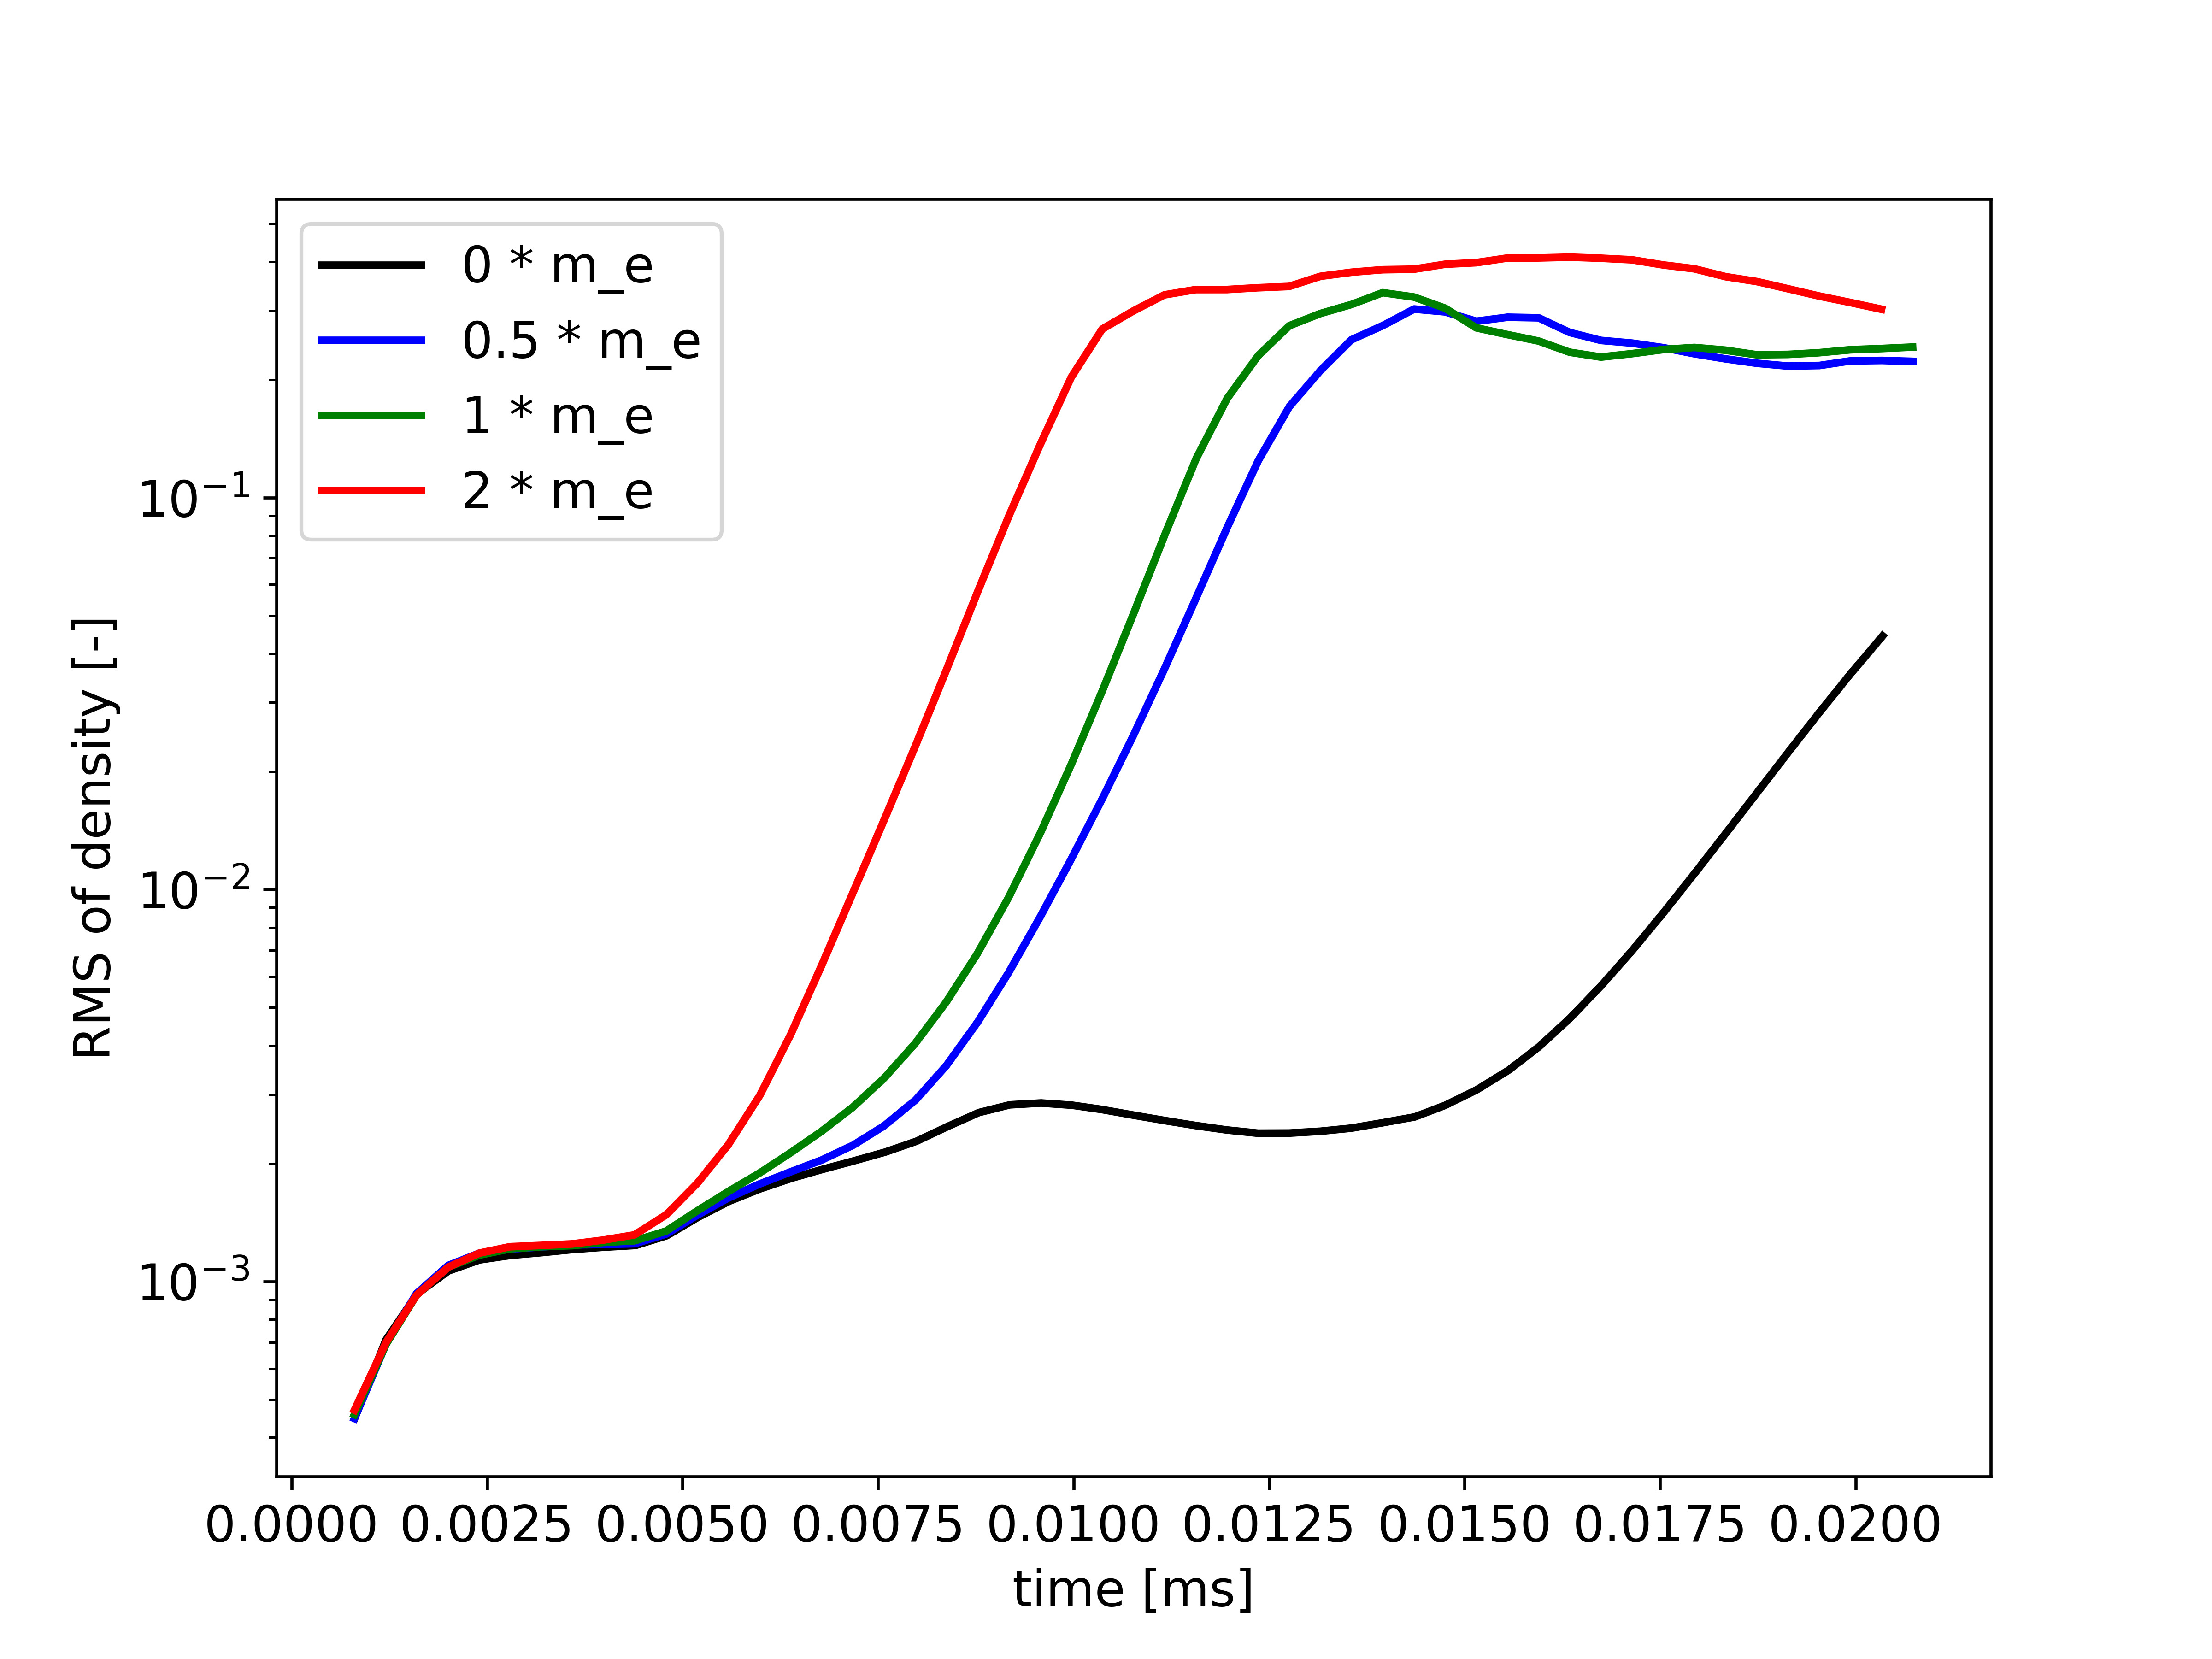
\includegraphics[width=1\textwidth]{schemes/RMSn_meScan.jpg}
		\subcaption{RMS of density $n_i$}
	\end{subfigure}
	\begin{subfigure}[t]{0.45\textwidth}
		\centering
		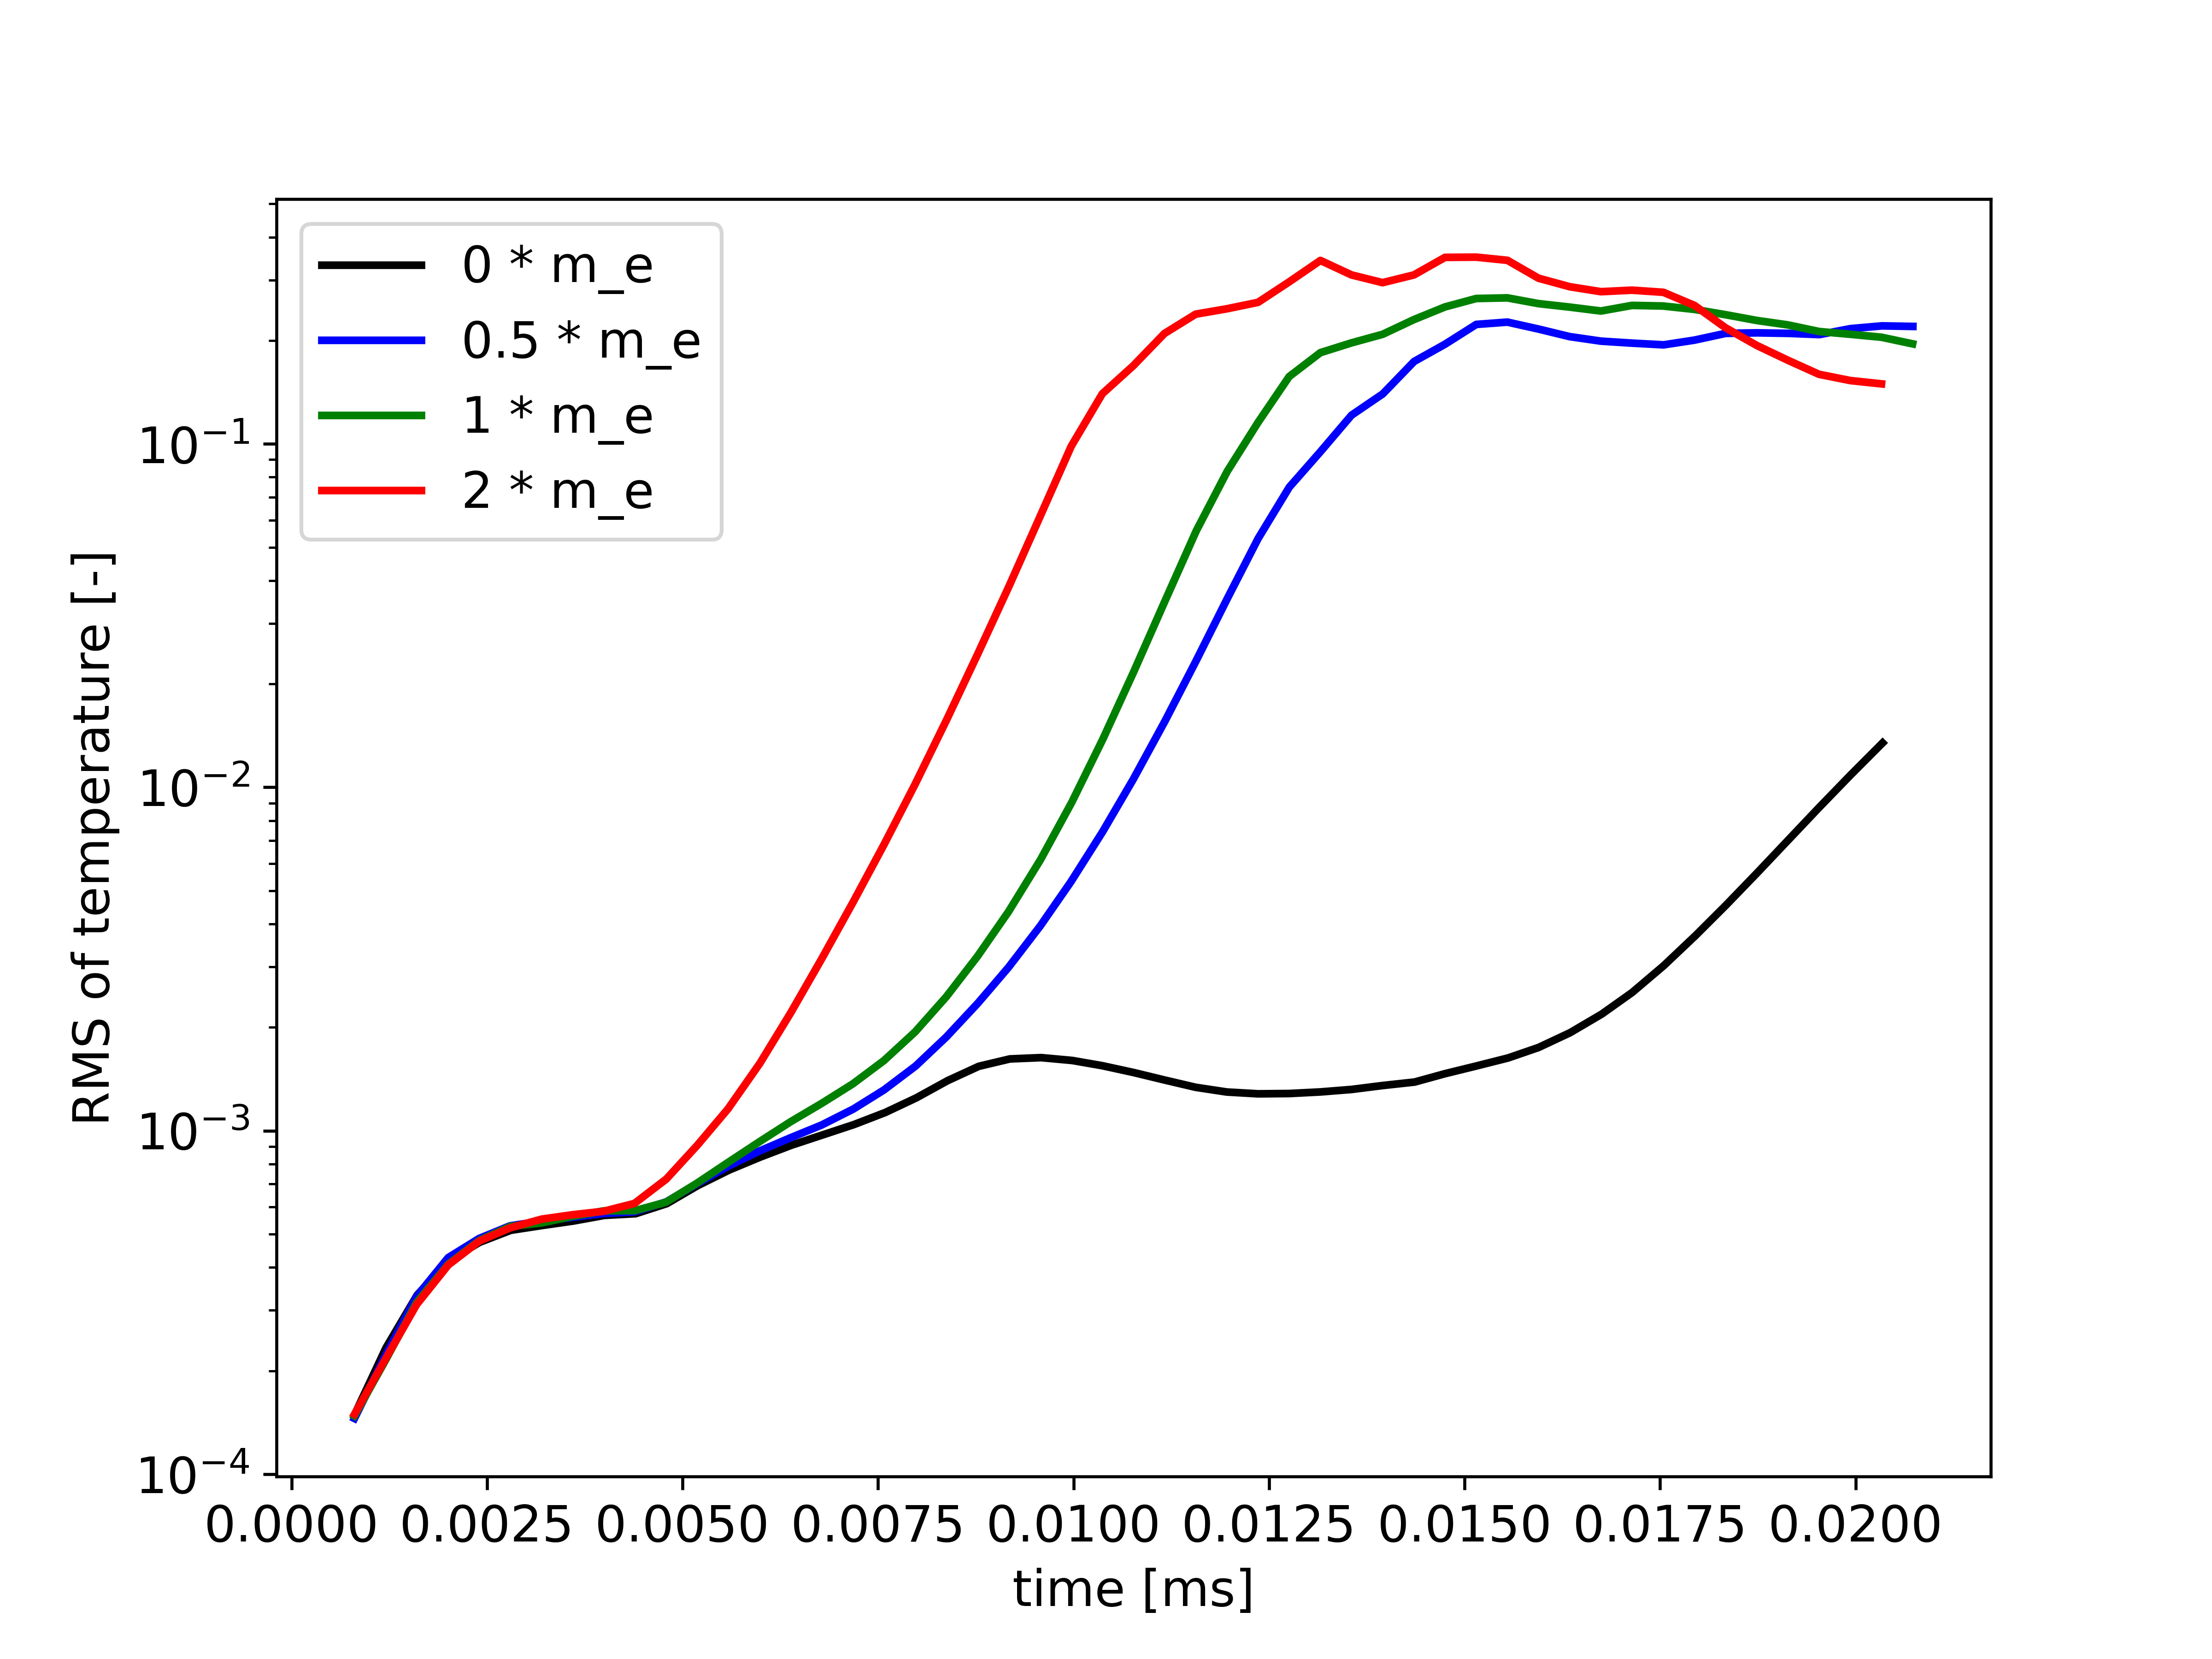
\includegraphics[width=1\textwidth]{schemes/RMST_meScan.jpg}
		\subcaption{RMS of temperature $T_i$}
	\end{subfigure}
	\caption{Evolution of the the perturbation intensity for different values of $m_e$. The electron mass is artificially increased and the 0 factor corresponds effectively to the electrostatic reference}
	\label{fig:CIRC_meScan}
\end{figure}



\subsubsection{Magnetic induction}

\begin{figure}[H]\centering
	\begin{subfigure}[t]{0.45\textwidth}
		\centering
		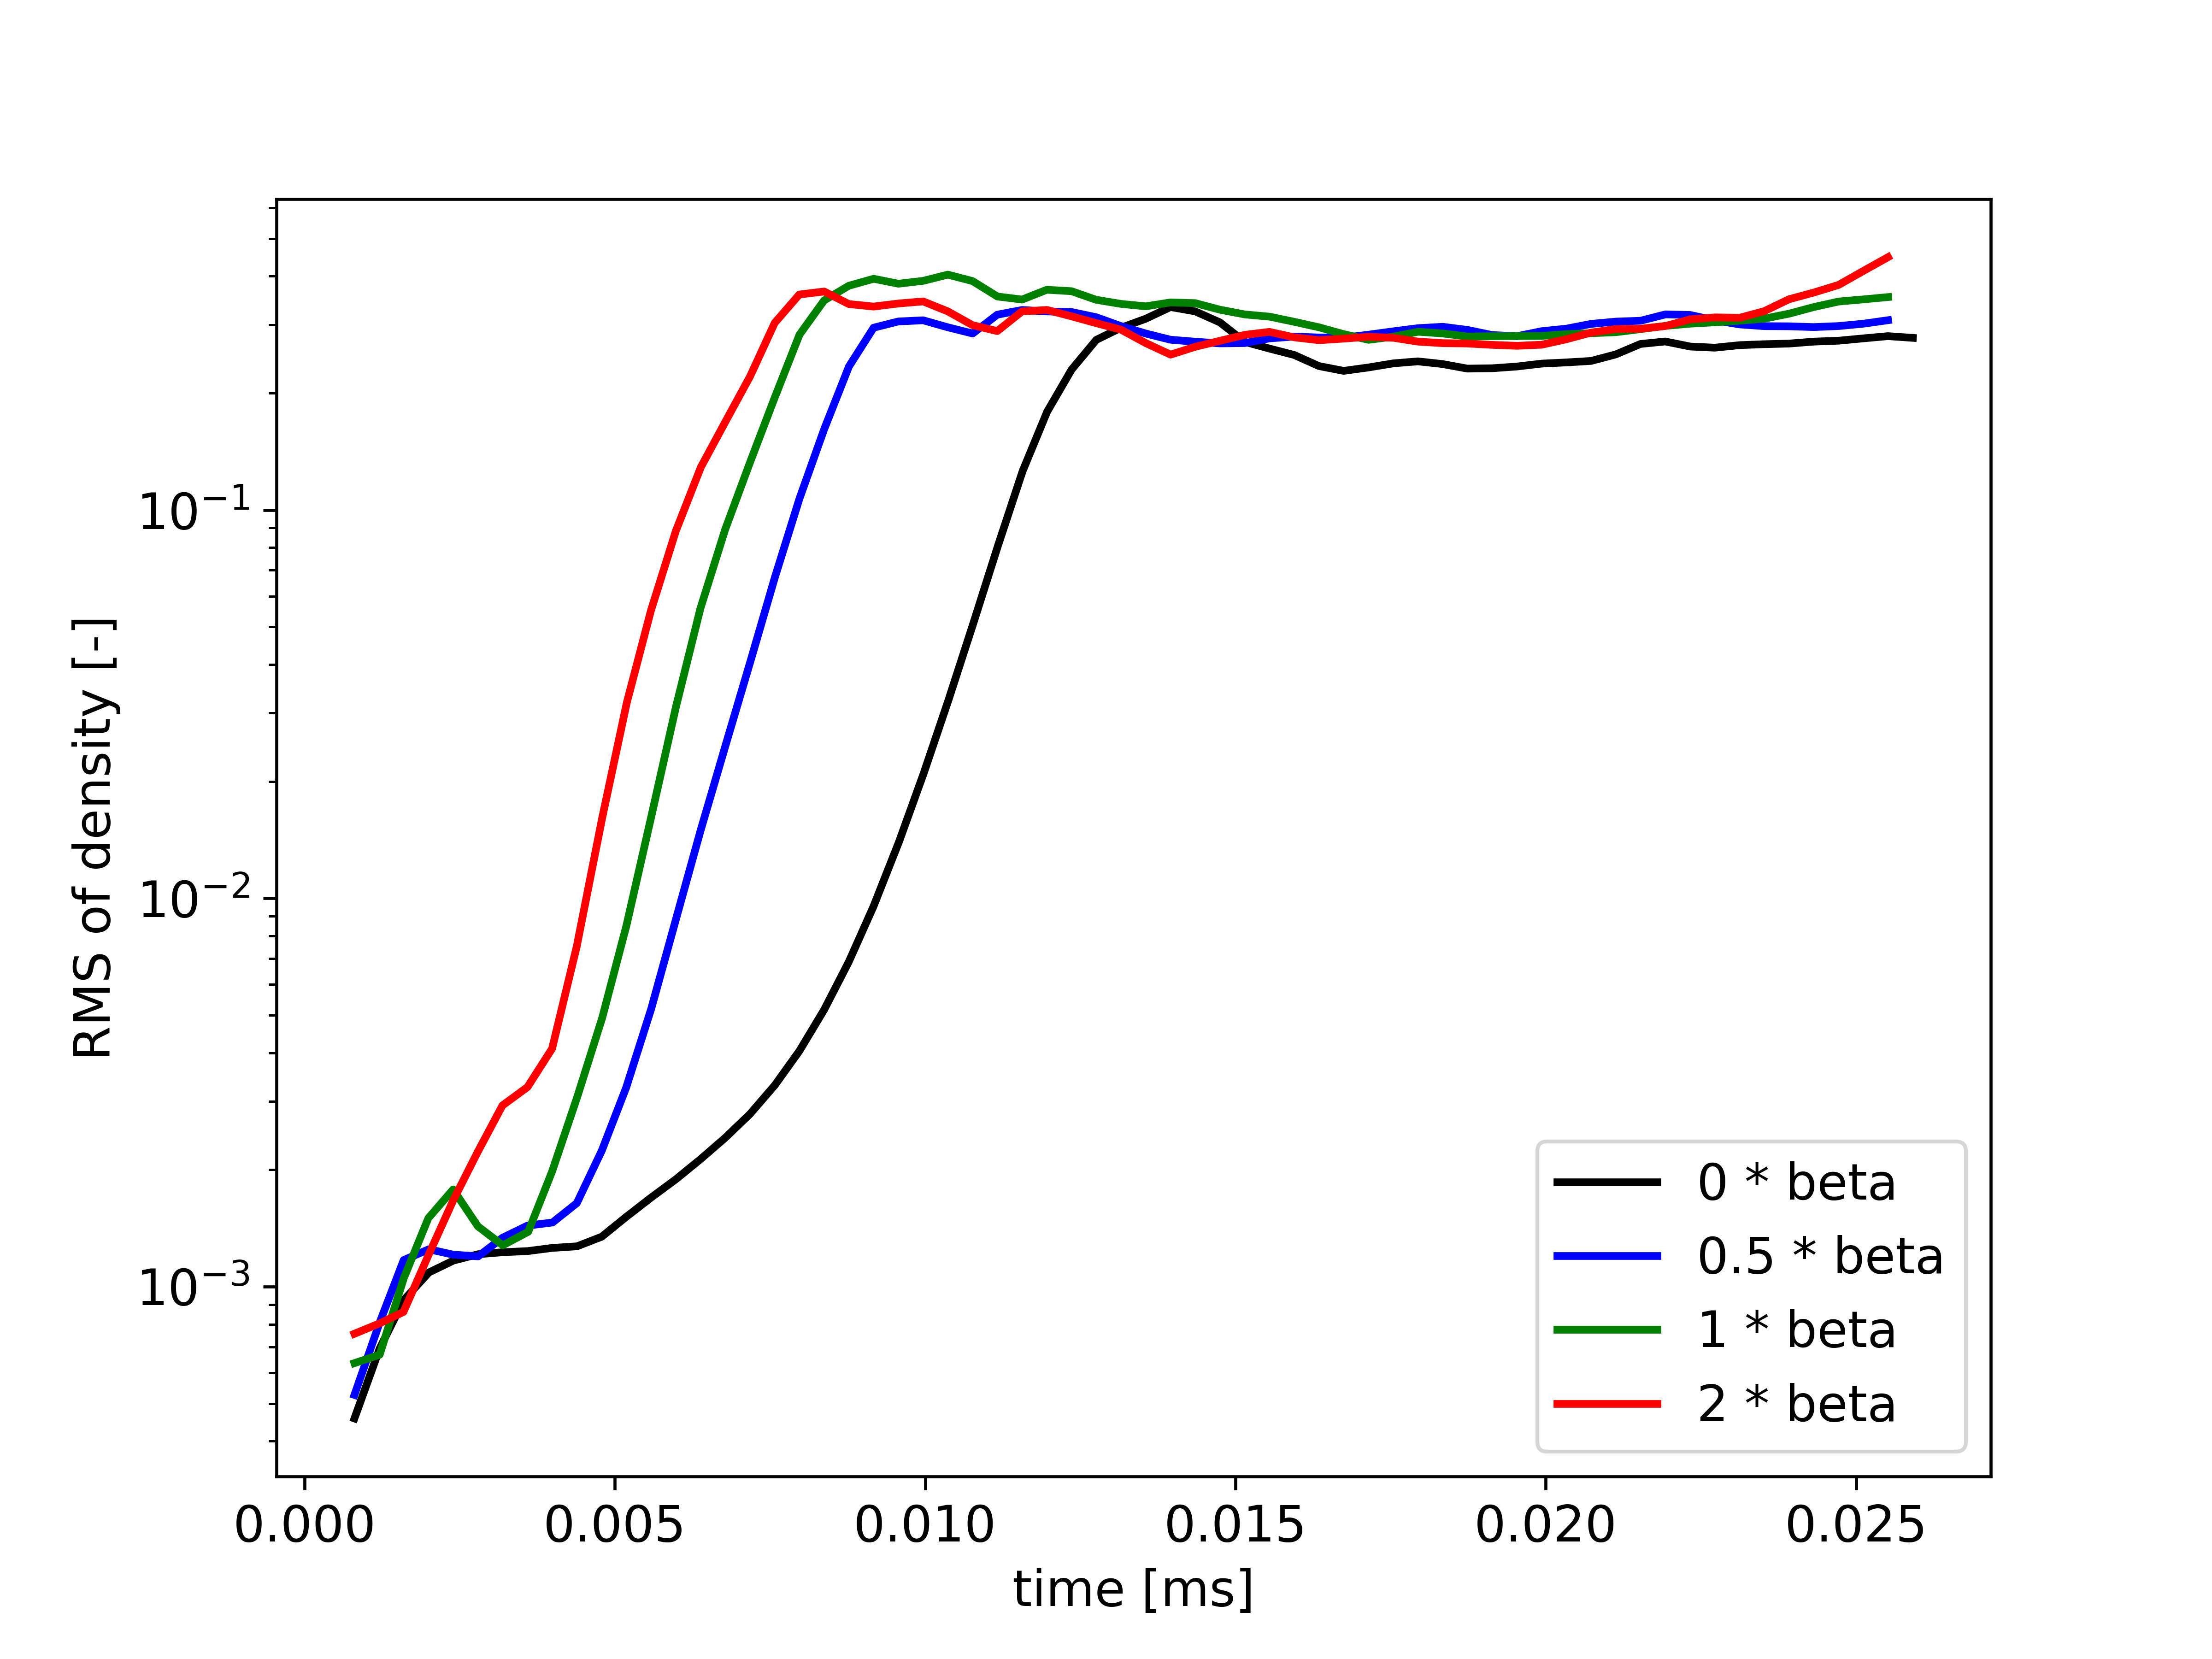
\includegraphics[width=1\textwidth]{schemes/RMSn_betaScan.jpg}
		\subcaption{RMS of density $n_i$}
	\end{subfigure}
	\begin{subfigure}[t]{0.45\textwidth}
		\centering
		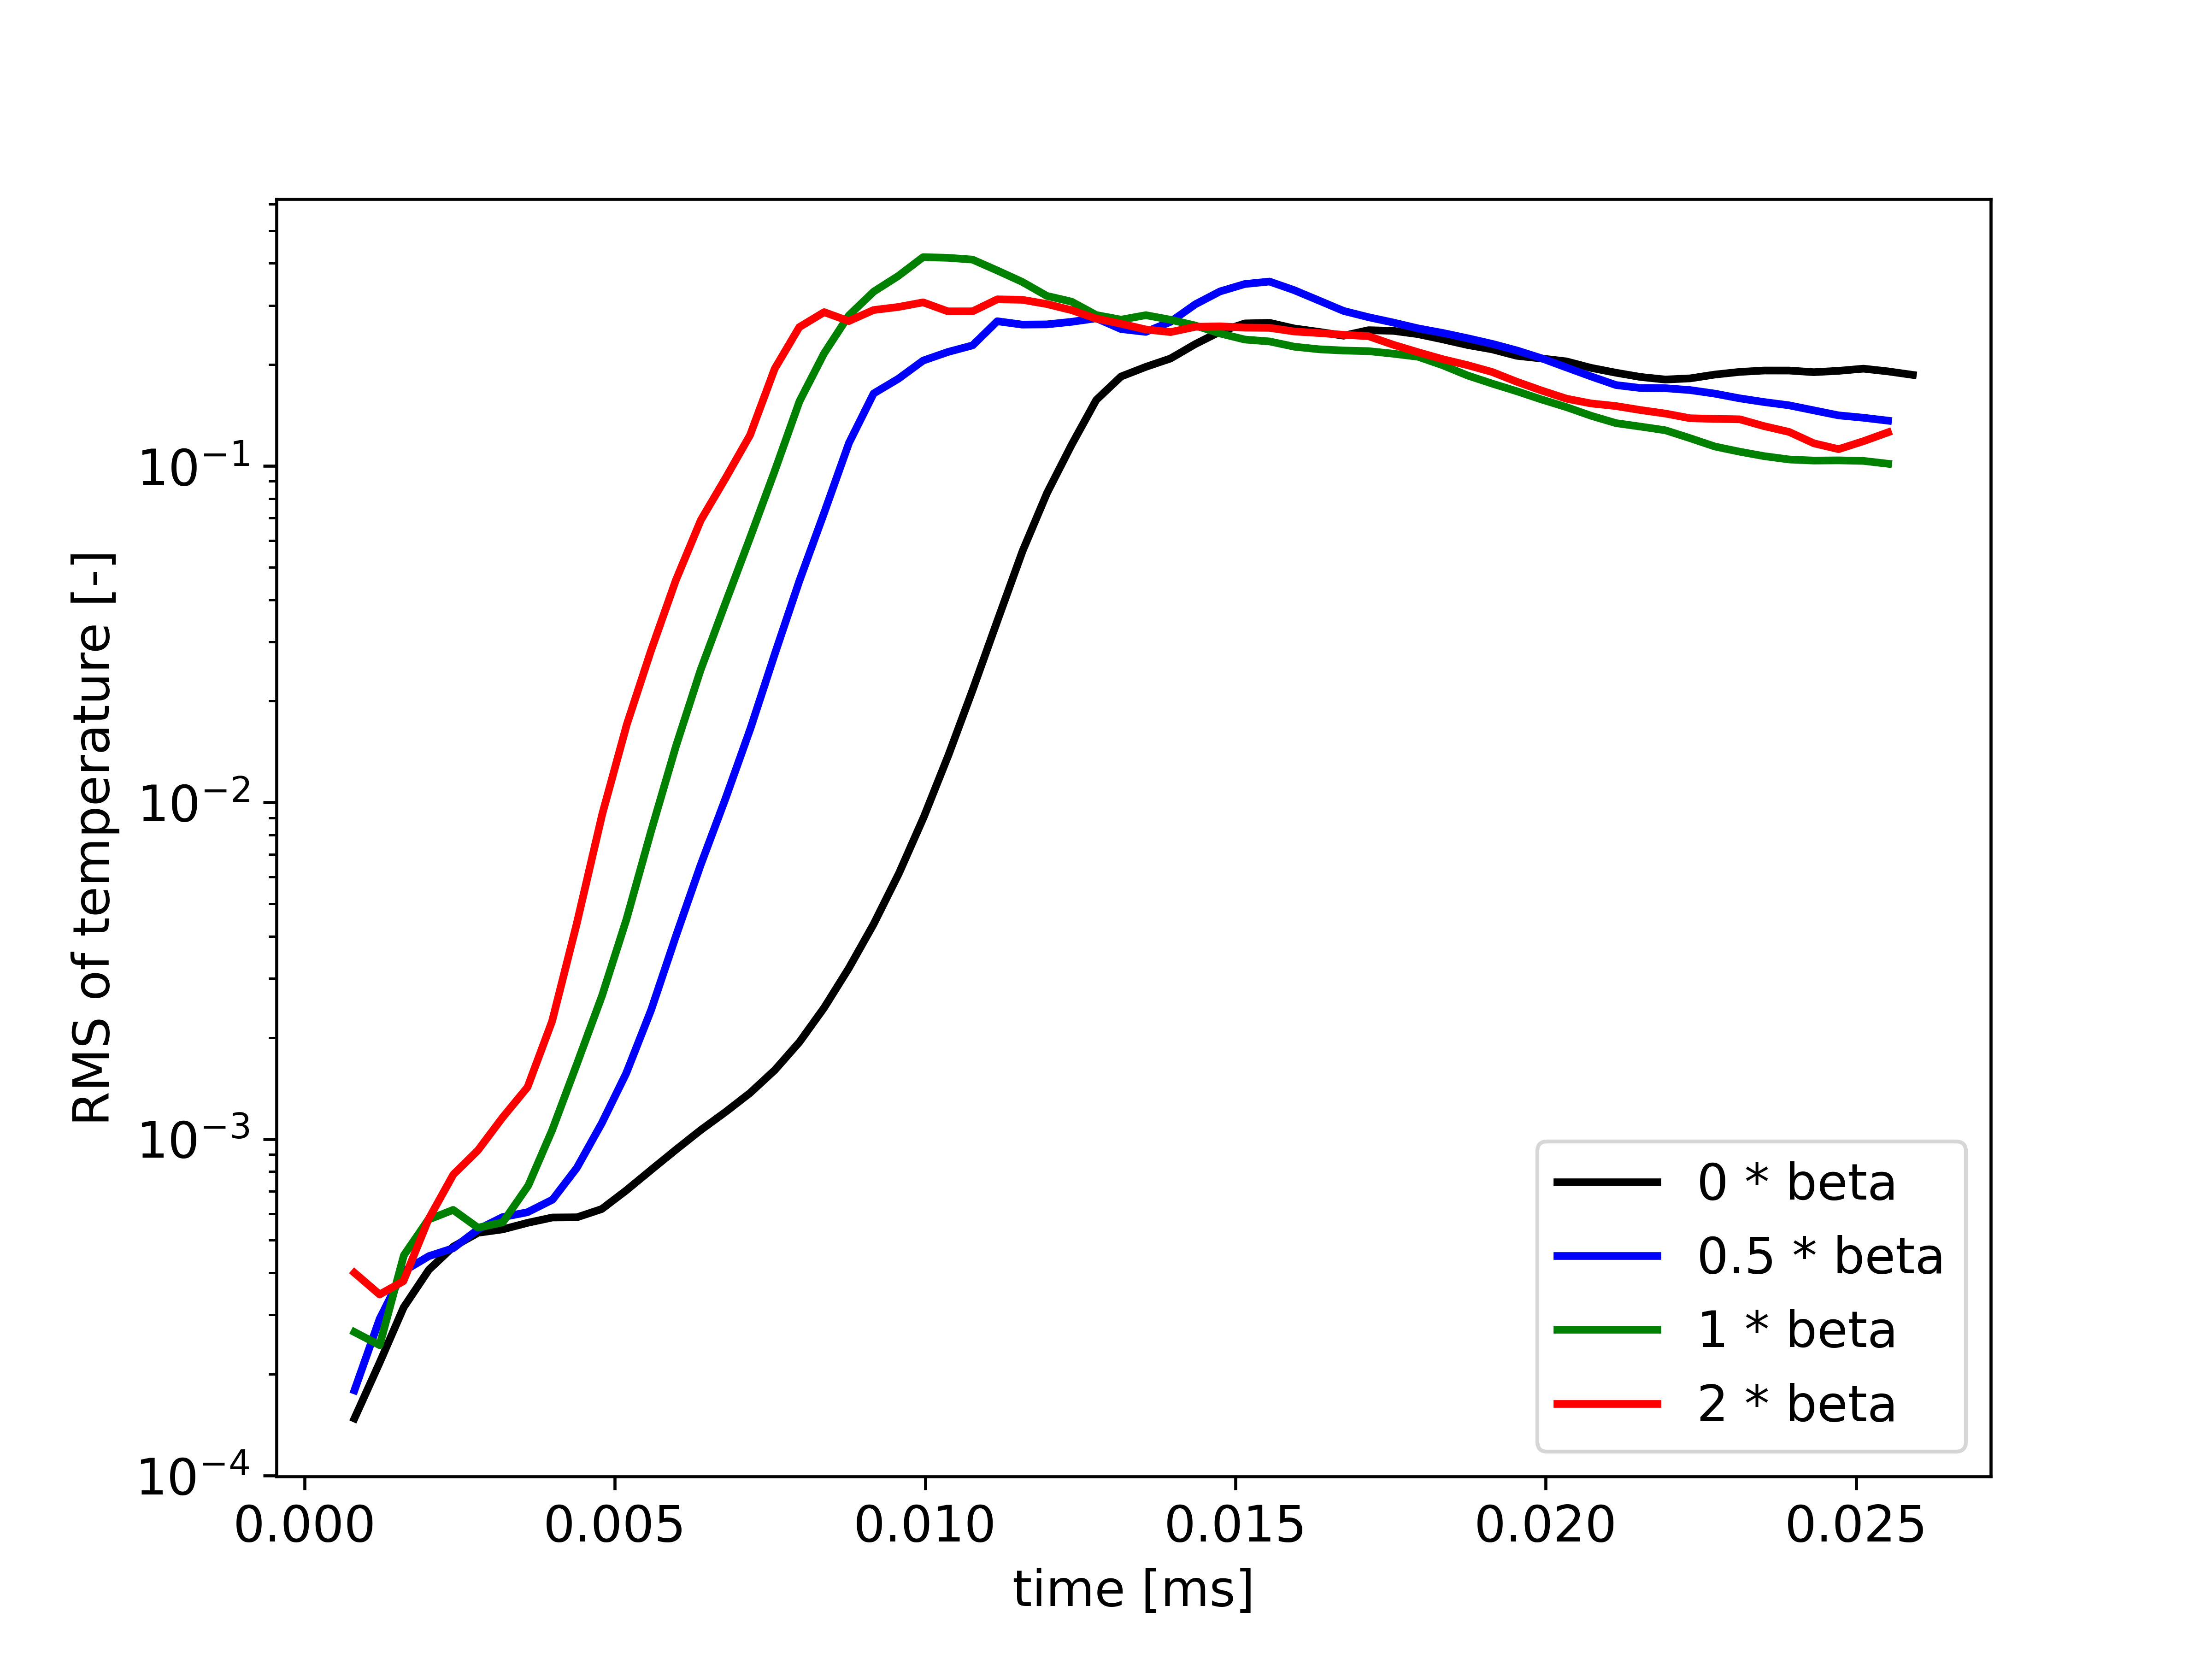
\includegraphics[width=1\textwidth]{schemes/RMST_betaScan.jpg}
		\subcaption{RMS of temperature $T_i$}
	\end{subfigure}
	\caption{Evolution of the the perturbation intensity for different values of $\beta$. The  is artificially increased and the 0 factor corresponds effectively to the electrostatic with electron inerita. The electron mass for all scenarios is physical (factor 1 in Fig. \ref{fig:CIRC_meScan}).}
	\label{fig:CIRC_betaScan}
\end{figure}



\subsection{Stabilization by flutter}







